\documentclass[../main.tex]{subfiles}
\graphicspath{{\subfix{../images/}}}

% Language setting
% Replace `english' with e.g. `spanish' to change the document language
\usepackage[english]{babel}

% Set page size and margins
% Replace `letterpaper' with `a4paper' for UK/EU standard size
\usepackage{geometry}

% Useful packages
\usepackage[utf8]{inputenc} % allow utf-8 input
\usepackage[T1]{fontenc}    % use 8-bit T1 fonts
\usepackage{hyperref}       % hyperlinks
\usepackage{url}            % simple URL typesetting
\usepackage{booktabs}       % professional-quality tables
\usepackage{amsfonts}       % blackboard math symbols
\usepackage{amsmath}
\usepackage{amssymb}
\usepackage{amsthm}
\usepackage{natbib}
\usepackage{nicefrac}       % compact symbols for 1/2, etc.
\usepackage{microtype}      % microtypography
\usepackage{xcolor}         % colors
\usepackage{graphicx}       % figures
\usepackage{enumitem}
\usepackage{tabularx}


\begin{document}

In addition to the works cited in the main paper, we make reference to the textbook \citep{foss2013introduction} throughout the proof. Many similar results about random variables are present in the textbook.

\subsubsection{Proof sketch and intuitions}

 The conditional expectation \(\mathbb E[V | X + V > t]\) is given by \(\frac{\int_{-\infty}^\infty vf_V(v)\text{Pr}(X>t-v)} {\int_{-\infty}^\infty f_V(v)\text{Pr}(X>t-v)}\), \footnote{We'll generally omit \(dx\) and \(dv\) terms in the interests of compactness and conciseness; the implied differentials should be pretty clear.}
 and we divide the integral in the numerator into 4 regions, showing that each region's effect on the conditional expectation of V is similar to that of the corresponding region in the unconditional expectation \(\mathbb E[V]\).

The regions are defined in terms of a slow-growing function \(h(t):\mathbb R \to \mathbb R_{\ge 0}\) such that the fiddly bounds on different pieces of the proof work out. Roughly, we want it to go to infinity so that \(|V|\) is likely to be less than \(h(t)\) in the limit, but grow slowly enough that the shape of \(V\)'s distribution within the interval \([-h(t),h(t)]\) doesn't change much after conditioning.

In Table \ref{table1}, we abbreviate the condition \(X+V>t\) as \(c\).

\begin{table}
\label{table1}
    \centering
    \begin{tabular}{|c|c|p{70mm}|}
    \hline \\
         Region
        &Why its effect on \(\mathbb E[V|c]\) is small
        & Explanation
    \\ \hline \\
        \(r_1=(-\infty,-h(t)]\)
        & \(\mathbb P[V\in r_1 | c]\) is too low  & In this region, \(|V| > h(t)\) and \(X > t + h(t)\), both of which are unlikely.
    \\ \hline \\
        \(r_2=(-h(t),h(t))\) 
        &  \(\mathbb E[V|V \in r_2, c] \approx \mathbb E[V|V \in r_2]\)
        & The tail distribution of X is too flat to change the shape of \(V\) 's distribution within this region.
    \\ \hline \\
        \(r_3\!=\![h(t),t\!-\!h(t)]\)
        & \(\mathbb P\left[ V \in r_3\ |\ c\right]\) is low, and \(V<t\).
        & There are increasing returns to each bit of optimization for X, so it's unlikely that both X and V have moderate values. \footnote{The diagrams in the previous post TODO show visually that when \(X\) and \(V\) are both heavy-tailed and \(t\) is large, most of the probability mass has \(X \approx 0\), \(V \approx t\) or vice versa.}
    \\ \hline \\
    \(r_4=(t-h(t),\infty)\) &  \(\mathbb P[V\in r_4 \ |\ c]\) is too low
        & X is heavier-tailed than V, so the condition that \(V > t-h(t)\) is much less likely than \(X > t - h(t)\) in \(r_2\).
    \\ \hline
    \end{tabular}
    \caption{A summary of the proof strategy for Theorem 5.}
\end{table}

\begin{figure}
    \centering
    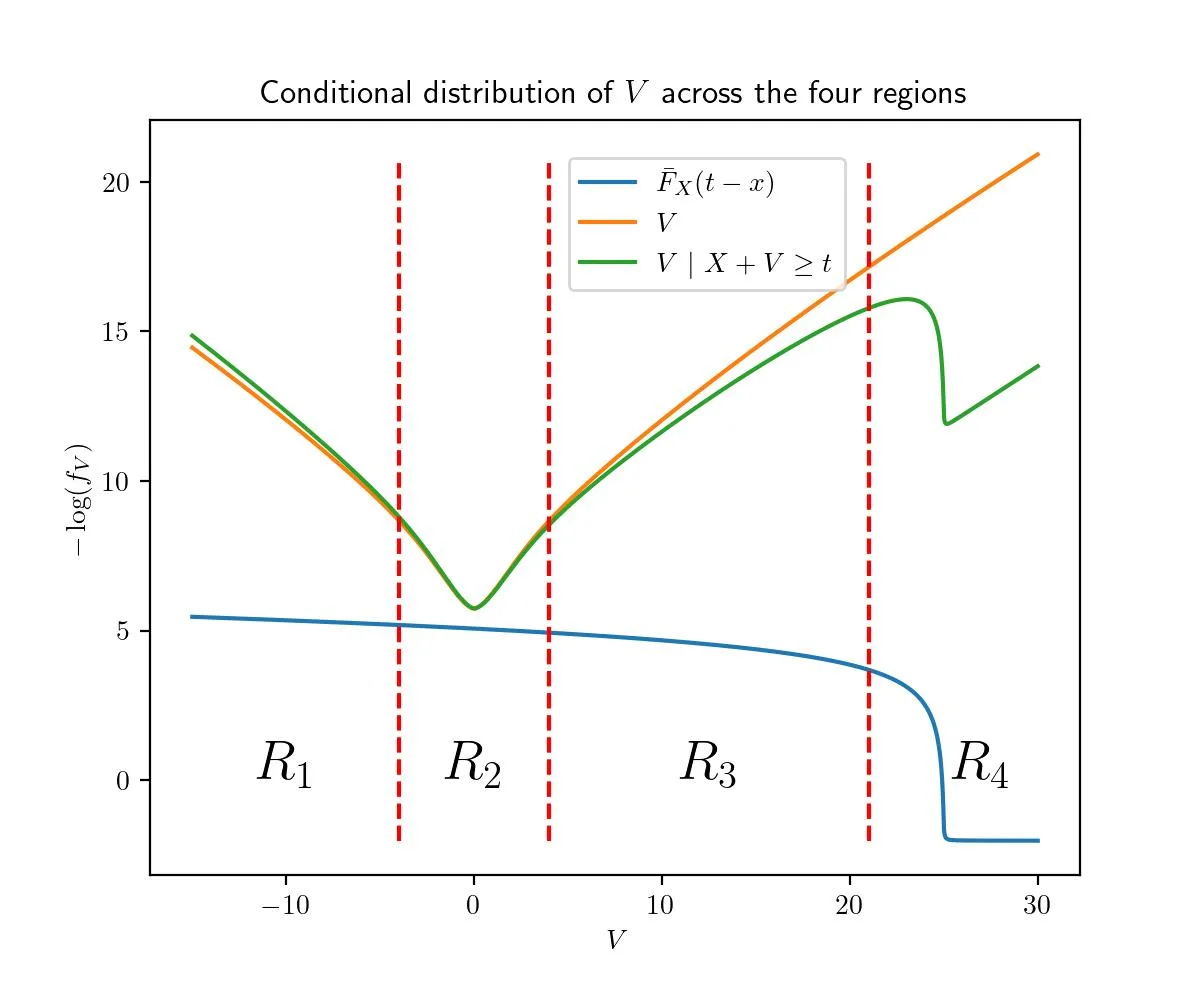
\includegraphics[width=0.5\linewidth]{supplementary/theorem5_diagram.png}
    \caption{A diagram showing the region boundaries at \(-h(t)\), \(h(t)\), and \(t-h(t)\) in an example where \(t=25\) and \(h(t)=4\), along with a negative log plot of the relevant distribution:}
    \label{fig:theorem5-diagram}
\end{figure}

Note that up to a constant vertical shift of normalization, the green curve is the pointwise sum of the blue and orange curves.

\subsubsection{Definitions}

To be more precise, we're going to make the following definitions and assumptions:

Let \(f_V(v)\) be the PDF of \(V\) at the value \(v\). We assume for convenience that \(f_V\) exists, is integrable, etc, though we suspect that this isn't necessary, and that one could work through a similar proof just referring to the tails of \(V\). We won't make this assumption for \(X\).
Let \(F_X(x)=\text{Pr}(X\le x)\) and \(\bar{F}_X(x)=\text{Pr}(X>x)\), similarly for \(F_V\) and \(\bar{F}_V\). 
Assume that
\begin{itemize}
    \item \(V\) has a finite mean: \(\int_{-\infty}^\infty vf_V(v)\,dv\) converges absolutely.
    \item \(X\) is subexponential.
\end{itemize}

Formally, this means that \(\lim_{x\to\infty}\frac{\text{Pr}(X_1+X_2>x)}{\text{Pr}(X>x)} = 2\). 
This occurs roughly whenever \(X\) has tails that are heavier than \(e^{-cx}\) for any \(c\) and is reasonably well-behaved; counterexamples to the claim "long-tailed implies subexponential" exist, but they're nontrivial to exhibit.
Examples of subexponential distributions include log-normal distributions, anything that decays like a power law, the Pareto distribution,and distributions with tails asymptotic to \(e^{-x^a}\) for any \(0<a<1\).

We require for \(V\) that its tail function is substantially lighter than X's, namely that \(\lim_{t\to\infty}\frac{t^p\bar F_V(t)}{\bar F_X(t)} = 0\) for some \(p > 1\). (This implies that \(\bar F_V(t) = O(\bar F_X(t) / t)\).)

With these definitions and assumptions, we can move on to the proof. 

The unnormalized PDF of \(V\) conditioned on \(X+V\ge t\) is given by \(f_V(v)\bar{F}_X(t-v)\). Its expectation is given by \(\frac{\int_{-\infty}^\infty vf_V(v)\bar{F}_X(t-v)} {\int_{-\infty}^\infty f_V(v)\bar{F}_X(t-v)}\).

Meanwhile, the unconditional expectation of V is given by \(\int_{-\infty}^\infty vf_V(v)\).

We'd like to show that these two expectations are equal in the limit for large \(t\). To do this, we'll introduce \(Q(v)=\frac{\bar{F}_X(t-v)}{\bar{F}_X(t)}\). (More pedantically, this should really be \(Q_t(v)\), which we'll occasionally use where it's helpful to remember that this is a function of \(t\).)

For a given value of \(t\), \(Q(v)\) is just a scaled version of \(\bar{F}_X(t-v)\), so the conditional expectation of \(V\) is given by \(\frac{\int_{-\infty}^\infty vf_V(v)Q(v)} {\int_{-\infty}^\infty f_V(v)Q(v)}\). But because \(Q(0)=1\), the numerator and denominator of this fraction are (for small \(v\) ) close to the unconditional expectation and \(1\), respectively.

We'll aim to show that for all \(\epsilon>0,\) we have for sufficiently large \(t\) that \(\left|\int_{-\infty}^\infty vf_V(v)Q_t(v) - \int_{-\infty}^\infty vf_V(v)\right|<\epsilon\) and \(\int_{-\infty}^\infty f_V(v)Q_t(v) \in [1-\epsilon,1+\epsilon]\), which implies (exercise) that the two expectations have limiting difference zero. But first we need some lemmas.

\subsubsection{Lemmas}

\begin{lemma}
 There is \(h(t)\) depending on \(F_X\) such that:
\begin{enumerate}[label=(\alph*)]
    \item \(\lim_{x\to\infty} h(t)=\infty\)
    \item \(\lim_{t \to\infty} t - h(t) = \infty\)
    \item \(\lim_{t\to\infty}\frac{\bar F_X(t-h(t))}{\bar F_X(t)}=1\)
    \item \(\lim_{t \to \infty} \sup_{|v| \le h(t)} |Q(v,t)-1| = 0\).
\end{enumerate}
\end{lemma}

\begin{proof}
 Lemma 2.19 from \citep{foss2013introduction} implies that if \(X\) is long-tailed (which it is, because subexponential implies long-tailed), then there is \(h(t)\) such that condition (a) holds and \(\bar F_X\) is \(h\)-insensitive; by Proposition 2.20 we can take \(h\) such that \(h(t) \le t/2\) for sufficiently large \(t\), implying condition (b). Conditions (c) and (d) follow from being \(h\)-insensitive.
 \end{proof}

\begin{lemma}
 Suppose that \(F_X\) is whole-line subexponential and \(h\) is chosen as in Lemma 1. Also suppose that \(\bar F_V(t) = O(\bar F_X(t) / t)\). Then \(Pr[X+V>t,\ V>h(t),\ X > h(t)] = o(\bar F_X(t)/t).\)
 \end{lemma}
 
\begin{proof}

 This is a slight variation on lemma 3.8 from \citep{foss2013introduction}, and follows from the proof of Lemma 2.37. Lemma 2.37 states that

\begin{quote}
    \textbf{Lemma 2.37.} Let $h$ be any increasing function on $\mathbb{R}^{+}$such that $h(x) \rightarrow \infty$. Then, for any distributions $F_1, F_2, G_1$, and $G_2$ on $\mathbb{R}$,
$$
\limsup _{x \rightarrow \infty} \frac{\mathbb{P}\left\{\xi_1+\eta_1>x, \xi_1>h(x), \eta_1>h(x)\right\}}{\mathbb{P}\left\{\xi_2+\eta_2>x, \xi_2>h(x), \eta_2>h(x)\right\}} \leq \limsup _{x \rightarrow \infty} \frac{\overline{F_1}(x)}{\overline{F_2}(x)} \cdot \limsup _{x \rightarrow \infty} \frac{\overline{G_1}(x)}{\overline{G_2}(x)},
$$
where $\xi_1, \xi_2, \eta_1$, and $\eta_2$ are independent random variables with respective distributions $F_1, F_2, G_1$ and $G_2$.
\end{quote}

but it is actually proved that \begin{multline}\mathbb{P}\left\{\xi_1+\eta_1>x, \xi_1>h(x), \eta_1>h(x)\right\} \leq \\ \sup_{z > h(x)} \frac{\overline{F_1}(z)}{\overline{F_2}(z)} \cdot \sup_{z > h(x)} \frac{\overline{G_1}(z)}{\overline{G_2}(z)} \cdot {\mathbb{P}\left\{\xi_2+\eta_2>x, \xi_2>h(x), \eta_2>h(x)\right\}}.\end{multline}

If we let \(F_1 = F_V, F_2=G_1=G_2=F_X\), then we get  \begin{multline} \mathbb{P}\left\{X+V>t, X>h(t), V>h(t) \right\}  \\ \le \sup_{z > h(t)} \frac{\bar F_V(z)}{\bar F_X(z)} \sup_{z > h(t)} \frac{\bar F_X(z)}{\bar F_X(z)} {\mathbb{P}\left\{X+X'>t, X>h(t), X'>h(t)\right\}}\\ = \sup_{z > h(t)} \frac{\bar F_V(z)}{\bar F_X(z)} {\mathbb{P}\left\{X+X'>t, X>h(t), X'>h(t)\right\}}\\ \end{multline}

where \(X,X' \sim F_X\). Multiplying by \(t\), we have

\begin{multline} t \mathbb{P}\left\{X\!+\!V>t, X\!>\!h(t), V\!>\!h(t) \right\} \le \sup_{z > h(t)} \frac{t\bar F_V(z)}{\bar F_X(z)} {\mathbb{P}\left\{X\!+\!X'>t, X\!>\!h(t), X'\!>\!h(t)\right\}}, \end{multline}

and because \(h(t) \to\infty\) as \(t \to\infty\) and \(\bar F_V(t) = O(\bar F_X(t) / t)\), we can say that for some \(c < \infty\), \(\lim_{t \to\infty} \sup_{z > h(t)} \frac{t\bar F_V(z)}{\bar F_X(z)} < c\). Therefore for sufficiently large t \(\mathbb{P}\left\{X+V>t, X>h(t), V>h(t) \right\} \leq \frac c t {\mathbb{P}\left\{X\!+\!X'>t, X\!>\!h(t), X'\!>\!h(t)\right\}}\). 

By Theorem 3.6, \(\mathbb{P}\left\{X\!+\!X'>t, X\!>\!h(t), X'\!>\!h(t)\right\}\) is \(o(\bar F_X(t))\), so the LHS is \(o(\bar F_X(t)/t)\) as desired.
\end{proof}

\subsubsection{Bounds on the numerator}

We want to show, for arbitrary \(\epsilon>0\), that \(\left|\int_{-\infty}^\infty vf_V(v)Q(v) - \int_{-\infty}^\infty vf_V(v)\right|<\epsilon\) in the limit as \(t\to\infty\). Since \(\left|\int_{-\infty}^\infty vf_V(v)Q(v) - \int_{-\infty}^\infty vf_V(v)\right| \le \int_{-\infty}^\infty \left|vf_V(v)(Q(v) - 1)\right| = \int_{-\infty}^\infty |v| \cdot f_V(v) \cdot |Q(v) - 1|\) it will suffice to show that the latter quantity is less than \(\epsilon\) for large \(t\).

We're going to show that \(\int_{-\infty}^\infty |v|\cdot f_V(v)\cdot |Q(v) - 1|\) is small by showing that the integral gets arbitrarily small on each of four pieces: \((-\infty,-h(t)]\), \((-h(t),h(t))\), \([h(t),t-h(t)]\), and \((t-h(t),\infty)\).

We'll handle these case by case (they'll get monotonically trickier).

\paragraph{Region 1: \texorpdfstring{\((-\infty,-h(t)]\)}{}}
 Since \(\int_{-\infty}^\infty vf_V(v)\) is absolutely convergent, for sufficiently large \(t\) we will have \(\int_{-\infty}^{-h(t)} |v|f_V(v) < \epsilon\), since \(h(t)\) goes to infinity by Lemma 1(a).

Since \(Q(v)\) is monotonically increasing and \(Q(0)=1\), we know that in this interval \(|Q(v)-1| = 1-Q(v)\).

So we have \(\int_{-\infty}^{-h(t)}|v|\cdot f_V(v) \cdot |Q(v)-1| = \int_{-\infty}^{-h(t)}|v|f_V(v)(1-Q(v)) < \int_{-\infty}^{-h(t)}|v|f_V(v) < \epsilon\) as desired.

\paragraph{Region 2: \texorpdfstring{\((-h(t),h(t))\)}{}}
 By lemma 1(d), \(h\) is such that for sufficiently large \(t\), \(|Q(v)-1|<\frac\epsilon{\int_{-\infty}^\infty |v|f_V(v)}\) on the interval \([-h(t),h(t)]\). (Note that the value of this upper bound depends only on \(V\) and \(\epsilon\), not on \(t\) or \(h\).) So we have \(\int_{-h(t)}^{h(t)}|v|f_V(v)|Q(v)-1| < \frac{\epsilon}{\int_{-\infty}^\infty|v|f_V(v)}\int_{-h(t)}^{h(t)}|v|f_V(v) < \frac{\epsilon}{\int_{-\infty}^\infty|v|f_V(v)}\int_{-\infty}^\infty|v|f_V(v) = \epsilon\).

\paragraph{Region 3: \texorpdfstring{\([h(t),t-h(t)]\)}{}}
 For the third part, we'd like to show that \(\int_{h(t)}^{t-h(t)}vf_V(v)(Q(v)-1)<\epsilon\). Since \(\int_{h(t)}^{t-h(t)}vf_V(v)(Q(v)-1) < \int_{h(t)}^{t-h(t)}tf_V(v)Q(v) = \frac t{\bar F_X(t)}\int_{h(t)}^{t-h(t)}f_V(v)\bar F_X(t-v)\) it would suffice to show that the latter expression becomes less than \(\epsilon\) for large \(t\), or equivalently that \(\int_{h(t)}^{t-h(t)}f_V(v)\bar F_X(t-v) = o\left(\frac{\bar F_X(t)}{t}\right)\).

The LHS in this expression is the unconditional probability that \(X+V>t\) and \(h(t)<V<t-h(t)\), but this event implies \(X+V>t, V>h(t)\), and \(X>h(t)\). So we can write

\begin{multline*}
\int_{h(t)}^{t-h(t)}f_V(v)\bar F_X(t-v) = Pr[X+V>t,\ h(t) < V < t - h(t)]
\\ < Pr[X+V>t,\ V > h(t),\ X > h(t)] = o(\bar F_X(t)/t)
\end{multline*}
by Lemma 2.

\paragraph{Region 4: \texorpdfstring{\((t-h(t),\infty)\)}{}}

For the fourth part, we'd like to show that \(\int_{t-h(t)}^\infty vf_V(v)Q(v) \to 0\) forlarge \(t\).

Since \(Q(v)=\frac{\bar F_X(t-v)}{\bar F_X(t)} < \frac 1{\bar F_X(t)}\), it would suffice to show \(\int_{t-h(t)}^\infty vf_V(v) = o(\bar F_X(t))\). But note that since \(\lim_{t\to\infty}\frac{\bar F_X(t-h(t))}{\bar F_X(t)} = 1\) by Lemma 1(c), this is equivalent to \(\int_{t-h(t)}^\infty vf_V(v) = o(\bar F_X(t-h(t)))\), which (by Lemma 1(b)) is equivalent to \(\int_t^\infty vf_V(v) = o(\bar F_X(t))\).

Note that \(\int_{t}^\infty vf_V(v) = t\int_{t}^\infty f_V(v) + \int_{t}^\infty (v-t)f_V(v) = t\bar F_V(t)+\int_{t}^\infty \bar F_V(v)\), so it will suffice to show that both terms in this sum are \(o(\bar F_X(t))\). 

The first term \(t \bar F_V(t)\) is \(o(\bar F_X(t))\) because we assumed \(\lim_{t\to\infty} \frac{t^p\bar F_V(t)}{\bar F_X(t)}=0\) for some \(p>1\).

For the second term, we have for the same reason \(\int_t^\infty \bar F_V(v) < \int_t^\infty \frac{\bar F_X(v)}{v^p} = \bar F_X(t)\int_t^\infty v^{-p} = \frac{t^{1-p}}{p-1}\bar F_X(t) = o(\bar F_X(t))\).

\subsubsection{Bounds on the denominator}

For the denominator, we want to show that \(\lim_{t\to\infty}\int_{-\infty}^\infty f_V(v)Q_t(v)=1=\int_{-\infty}^\infty f_V(v)\), so it'll suffice to show \(|\int_{-\infty}^\infty f_V(v)(Q_t(v)-1)|=o(1)\) as \(t\to\infty\). Again, we'll break up this integral into pieces, though they'll be more straightforward than last time. We'll look at \((-\infty,-h(t))\), \([-h(t),h(t)]\), and \((h(t),\infty)\).

\begin{itemize}
    \item \(|\int_{-\infty}^{-h(t)}f_V(v)(Q(v)-1)|=\int_{-\infty}^{-h(t)}f_V(v)(1-Q(v))<\int_{-\infty}^{-h(t)}f_V(v)\).
    \begin{itemize}
        \item But since \(h(t)\) goes to infinity, this left tail of the integral will contain less and less of \(V\) 's probability mass as $t$ increases.
    \end{itemize}
    \item \(|\int_{-h(t)}^{h(t)}f_V(v)(Q(v)-1)|\le\int_{-h(t)}^{h(t)}f_V(v)|Q(v)-1|\)
    \item \(\le \sup_{|v| \le h(t)} |Q(v,t)-1|\int_{-h(t)}^{h(t)}f_V(v)\le \sup_{|v| \le h(t)} |Q(v,t)-1|\)
    \begin{itemize}
        \item By Lemma 1(d) we know that this goes to zero for large \(t\).
    \end{itemize}
    \item \(|\int_{h(t)}^\infty f_V(v)(Q(v)-1)| = \int_{h(t)}^\infty f_V(v)(Q(v)-1) < \int_{h(t)}^\infty f_V(v)Q(v)\).
\end{itemize}

But for sufficiently large \(t\) we have \(h(t)>1\), so we obtain
 \(\int_{h(t)}^\infty f_V(v)Q(v)<\int_{h(t)}^\infty v f_V(v)Q(v) < \int_{-\infty}^\infty v f_V(v)Q(v) = o(1)\) 
by the results of the previous section. This completes the proof.

\end{document}